\section{Background in Wireless Networks}
\label{section:bgd_wlan}

In this chapter, the origins and the motivation underneath \gls{wifi} is exposed. The different authentication and encryption protocols are detailed, as defined by the \gls{ieee}, and have their security problems explained.

The research covers Open System and \gls{weo} standards, for unauthenticated or open networks; \gls{wep}, \gls{wpa}, \gls{wpa}2, and \gls{wpa}3 standards, for authenticated or closed networks; and \gls{wps} and \gls{wec} standards, for quick setup networks.

The knowledge acquired in this chapter is later used for the security assessment of the \glspl{cpe} and to better understand the impact of the configurations set.

\subsection{IEEE 802.11 and Wi-Fi}

\gls{ieee} 802.11 is a working group, part of the \gls{ieee} \gls{lmsc}, that develops and maintains networking standards and recommended practices for \gls{wlan} \cite{about_ieee_p80211}. The first version of its standard was released in 1997 and operated at a 2.4 \gls{G}\gls{Hz} frequency, allowing data to be transmitted up to 2 \gls{M}\gls{b}\gls{ps}.

The original standard was quickly superseded by the \gls{ieee} 802.11b amendment. Published in 1999, it increased the maximum transfer rate of the standard to 11 \gls{M}\gls{b}\gls{ps} while staying in the 2.4 \gls{G}\gls{Hz} band.

In the same year, companies joined forces together to certify interoperability of products implementing the \gls{ieee} 802.11 standard and to promote it as the global \gls{wlan} standard across all market segments. The \gls{weca} was born with that mission \cite{weca_mission}.

For months, \gls{weca} worked closely with several vendors of \gls{ieee} 802.11b equipment to develop an interoperability testbed for the standard. The work was complete in February 2000 and \gls{weca} members were able to submit their products against the test matrix. Upon success, the product would receive the \gls{wifi} CERTIFIED\textsuperscript{TM} seal and the company would be allowed to use the \gls{wifi}\textsuperscript{TM} logo on the device’s advertising and packaging. The seal indicates that the product "met industry-agreed standards for interoperability, security, and a range of application specific protocols" and works with any other devices that also bear the symbol \cite{wifi_certification}. In 2002, \gls{weca} changed its name to \gls{wifi} Alliance.

\begin{table}[h]
    \makebox[\linewidth]{
        \begin{tabular}{c|c}
            \thead{\gls{ieee} 802.11 Amendment} & \thead{\gls{wifi} Generation} \\
            \hline
            802.11b & \gls{wifi} 1 \\
            802.11a & \gls{wifi} 2 \\
            802.11g & \gls{wifi} 3 \\
            802.11n & \gls{wifi} 4 \\
            802.11ac & \gls{wifi} 5 \\
            802.11ax & \gls{wifi} 6 \\
        \end{tabular}
    }
    \caption{\gls{ieee} 802.11 Amendment to \gls{wifi} Generation mapping}
    \label{table:map_80211_wifi}
\end{table}

In 2018, the \gls{wifi} Alliance introduced a new designation to identify the \gls{wifi} generations \cite{wifi6_introduction}, moving away from the traditional \gls{ieee} 802.11 amendment names and adopting a simpler numerical sequence scheme as shown in Table \ref{table:map_80211_wifi}.

\FloatBarrier

\subsection{Open Network Standards}
\subsubsection{Open System}

The Open System authentication is essentially a null authentication algorithm \cite{ieee_80211_2020}. Any wireless client may become authenticated if the target of the request is configured to use this kind of authentication, although the recipient is not required to accept the authentication request and may decline it.

\subsubsection{Wi-Fi Enhanced Open}

The new security standard, was introduced in 2018 and intends to replace the Open System authentication for public networks. Based on the \gls{owe} \cite{rfc8110}, its main difference is the introduction of a privacy layer that encrypts traffic between the client and the station \cite{weo_introduction}.


\subsection{Protected Network Standards}
\subsubsection{WEP}

The \gls{wep} algorithm is part of the original \gls{ieee} 802.11 standard and was intended to avoid eavesdropping and ensure privacy for those connected to a wireless network \cite{ieee_80211_2020}.

It relies on a secret that is known by the station and has been delivered to the wireless client, presumably via a secure channel, to accept or decline the authentication request. An encrypted challenge is sent to the client, which decrypts it using the shared key and sends the decrypted challenge back to the station, proving that it knows the password, thus should be authenticated successfully.

\paragraph{Algorithm}

\begin{figure}[h]
    \centering
    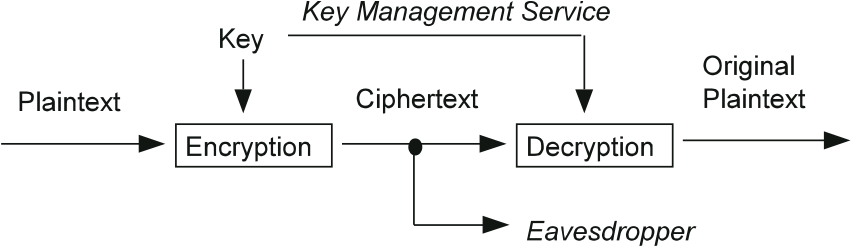
\includegraphics[width=\linewidth]{contents/background-in-wireless-networks/protected-network-standards/wep/algorithm/a-confidential-data-channel.png}
    \caption{A Confidential Data Channel}
    {Source: \cite{ieee_80211_2020}}
    \label{figure:ieee80211_figure43}
\end{figure}

The algorithm \cite{ieee_80211_2020} uses a key sequence produced by a \gls{prng} to encrypt and decrypt data, establishing a secure channel as shown in Figure \ref{figure:ieee80211_figure43}. The \gls{prng} used by \gls{wep} requires a 64-bit or 128-bit seed to initialize its initial state and derive the associated keystream. The \gls{wep} \gls{sk}, either 40 bits (\gls{wep}-40) or 104 bits (\gls{wep}-104) in size, and the \gls{iv}, 24 bits long, are concatenated and used as the seed for the \gls{prng}. The \gls{iv} content is random and its role is to avoid the \gls{prng} to be initialized with the same seed more than once, preventing the data from being encrypted with an already known key sequence.

The \gls{ia} is used to detect if the message sent via the wireless network was corrupted and possibly tempered with on transport, it takes the plaintext as input and produces 32 bits as the \gls{icv}.

\begin{figure}[h]
    \centering
    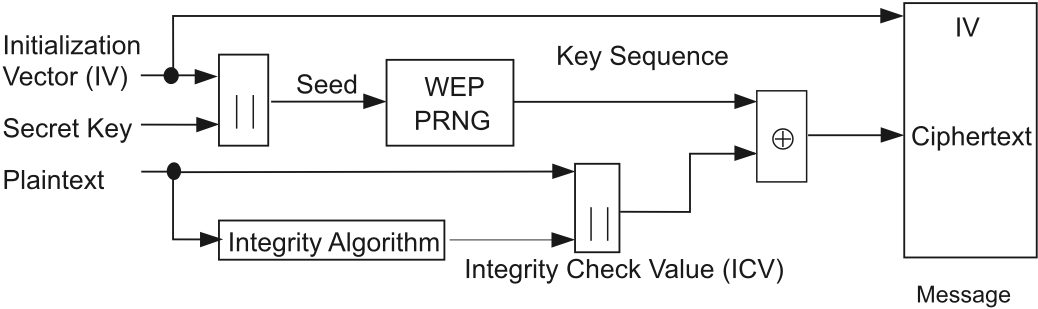
\includegraphics[width=\linewidth]{contents/background-in-wireless-networks/protected-network-standards/wep/algorithm/wep-encipherment-block-diagram.png}
    \caption{\gls{wep} Encipherment Block Diagram}
    {Source: \cite{ieee_80211_2020}}
    \label{figure:ieee80211_figure44}
\end{figure}

As illustrated on Figure \ref{figure:ieee80211_figure44}, to encrypt a message, the algorithm requires the \gls{sk}, the \gls{iv}, and the plaintext. First, the \gls{sk} and the \gls{iv} are fed to the \gls{prng}, and \gls{N} bits from the keystream are stored in \gls{KS}, where \gls{N} is the length of the plaintext added by the size of the \gls{icv}. Then the plaintext is fed to the \gls{ia} and the output is stored in \gls{icv}. The plaintext is concatenated with the \gls{icv} and XORed with \gls{KS}, resulting in the ciphertext. Finally, the \gls{iv} is concatenated with the ciphertext and returned as the output of the algorithm, the \gls{mpdu}.

\begin{figure}[h]
    \centering
    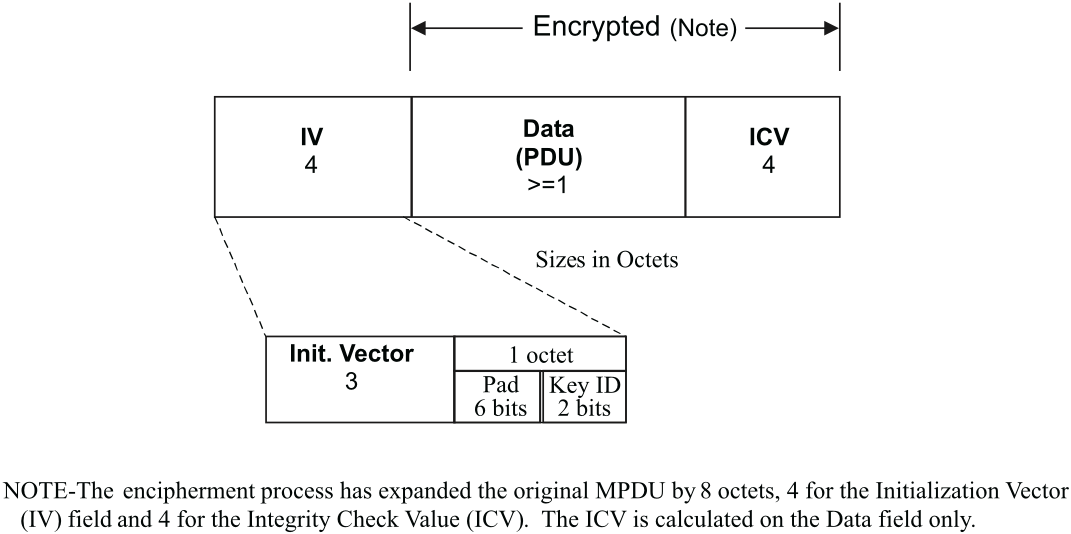
\includegraphics[width=\linewidth]{contents/background-in-wireless-networks/protected-network-standards/wep/algorithm/construction-of-expanded-wep-mpdu.png}
    \caption{Construction of Expanded \gls{wep} \gls{mpdu}}
    {Source: \cite{ieee_80211_2020}}
    \label{figure:ieee80211_figure46}
\end{figure}

Figure \ref{figure:ieee80211_figure46} shows the encrypted \gls{mpdu} as constructed by the \gls{wep} algorithm. It is transmitted over the wireless connection and then decrypted by the receiver. To decrypt the \gls{mpdu}, only the \gls{sk} is required. So the confidentiality of the data channel established using \gls{wep} essentially relies on the secrecy of the shared key.

\begin{figure}[h]
    \centering
    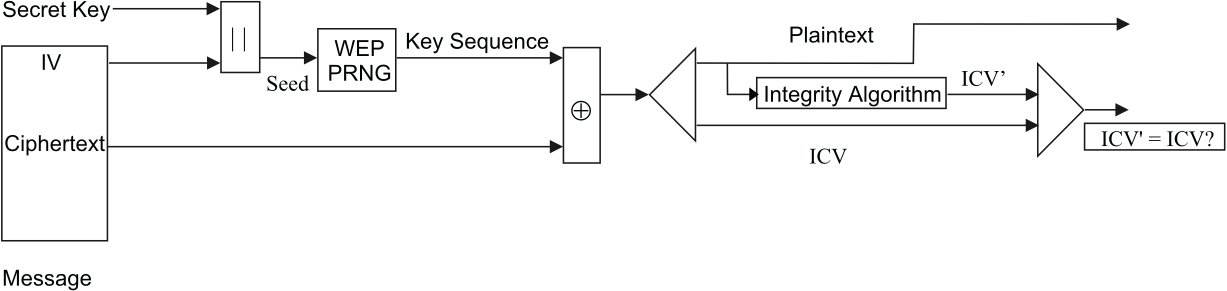
\includegraphics[width=\linewidth]{contents/background-in-wireless-networks/protected-network-standards/wep/algorithm/wep-decipherment-block-diagram.png}
    \caption{\gls{wep} Decipherment Block Diagram}
    {Source: \cite{ieee_80211_2020}}
    \label{figure:ieee80211_figure45}
\end{figure}

The decryption algorithm, as represented by Figure \ref{figure:ieee80211_figure45}, receives the \gls{sk} and the \gls{mpdu} to be decrypted. First, the \gls{iv} is extracted from the first 24 bytes of the \gls{mpdu} and appended to the \gls{sk}, resulting in the seed for the \gls{prng}. Then \gls{N} bits are consumed from the keystream and stored in \gls{KS}, \gls{N} is the length of the ciphertext and \gls{sk} the key sequence produced. The ciphertext is XORed with \gls{KS}, recovering the plaintext concatenated with the \gls{icv}. Finally, the plaintext is fed to the \gls{ia}, calculating \gls{icv}’. If the values of the extracted \gls{icv} and \gls{icv}’ are the same, the plaintext is successfully returned as the output of the algorithm. Otherwise, the \gls{mpdu} was corrupted and an error is sent to the \gls{mac} management.

\FloatBarrier

\paragraph{Security}

A compromise was made on the \gls{tkip} design to make possible its use on legacy \gls{wep} hardware. The forgery attacks were mitigated with the introduction of the Michael algorithm, but, due to computing power constraints, while blocking the forged packets it would cause a denial of service on the network \cite{ieee_80211_2020}.

As \gls{tkip} just encapsulates the \gls{wep} algorithm, it still relies on the security of the \gls{rc4} \gls{prng}. It was found that the keystream generated by \gls{rc4} is biased towards certain sequences and it made practical attacks against \gls{wpa}-\gls{tkip} networks within an hour \cite{rc4nomore}. The attacker would establish a \gls{tcp} connection with some victim on the network and would repeatedly send identical packets particularly sized with a well-known content over the connection. Then the wireless traffic was captured and filtered to only what would likely be an attacker's packet. Ciphertext statistics were extracted and plaintext likelihoods calculated using a combination of the \gls{fm} and \gls{absab} biases. Finally, the \gls{mic} key is derived from one of the candidates with the correct \gls{icv}, allowing any other packet of the victim to be fully decrypted.


\subsubsection{WPA}

The \gls{wpa} is a security protocol based on a draft of the \gls{ieee} 802.11i amendment. It was pushed by the \gls{wifi} Alliance in 2003 as an intermediate solution to the weaknesses of the \gls{wep} algorithm \cite{wifi_state}, allowing manufacturers to patch existing \gls{wep} devices with a safer authentication mechanism while maintaining interoperability. Since its conception, it was meant to be replaced as soon as the \gls{ieee} 802.11i amendment was published in its definitive form \cite{wpa_whitepaper}.

\gls{wpa} moved away from the 40-bit and 104-bit \gls{wep} keys and adopted two new authentication methods. \gls{wpa}-Personal uses a human-readable passphrase as proof of knowledge to authenticate clients. While \gls{wpa}-Enterprise relies on the \gls{ieee} 802.1X standard to authenticate clients on a remote server using one the \gls{eap} \cite{wpa_whitepaper}. Both authentication mechanisms result in the \gls{pmk}, a key that is used to derive other keys used internally by \gls{wpa} as foundation for its privacy protocols.

\paragraph{PSK}

The \gls{psk} is the authentication protocol of \gls{wpa}-Personal networks \cite{wifi_state}. It derives a 256-bit key \gls{DK} using the \gls{pbkdf2} algorithm \cite{rfc8018} from a sequence \gls{P} of 8 to 63 \gls{ascii}-encoded characters, between ' ' (32) and '$\sim$' (126) \cite{ieee_80211_2020}. On \gls{pbkdf2} invocation, the \gls{ssid} of the network is used as the salt \gls{S}, the iteration count \gls{c} is set to 4096, and the length \gls{dkLen} of \gls{DK} is given in bytes.

\[ \gls{DK} = \gls{pbkdf2}(\gls{P}, \gls{S}, \gls{c}, \gls{dkLen}) \]
\[ \therefore \]
\[ \gls{psk} = \gls{pbkdf2}(\gls{P}, \gls{ssid}, 4096, 256 / 8) \]

\paragraph{TKIP}

The \gls{tkip} is a cipher suite designed to enhance \gls{wep} on existing hardware when \gls{wpa} authentication is configured \cite{ieee_80211_2020}. \gls{tkip} encapsulates the original \gls{wep} algorithm to address all security problems known at the time while complying with the first generation stations' constraint of 4 million instructions per second, about 5 instructions per byte processed.

The \gls{mic} was introduced to detect forgery attacks. It is calculated with the Michael algorithm, that due to the computing constraints, couldn't provide the level of effectiveness desired and was complemented with countermeasures on a latter step of \gls{tkip} \cite{ieee_80211_2020}. The Michael algorithm relies on a key for authentication purposes, either a single 128-bit key is used by both nodes for encryption and decryption or each node has its 64-bit key for encryption, which is shared with the other node for decryption.

The frame order started to be enforced via the \gls{tkip} Sequence Counter to avoid replay attacks. Any \gls{mpdu} received out of sequence is ignored.

\begin{figure}[h]
    \centering
    
\includegraphics[width=\linewidth]{contents/background-in-wireless-networks/protected-network-standards/wpa/tkip/construction-of-expanded-tkip-mpdu.png}
    \caption{Construction of Expanded \gls{tkip} \gls{mpdu}}
    {Source: \cite{ieee_80211_2020}}
    \label{figure:ieee80211_figure43e}
\end{figure}

The original \gls{wep} \gls{mpdu} format was extended, as shown in Figure \ref{figure:ieee80211_figure43e}, to accommodate additional information required by \gls{tkip}, the \gls{eiv} and the \gls{mic}. The \gls{tkip} \gls{eiv} field is placed right after the original \gls{wep} \gls{iv} field and adds an extra 4 octets to the \gls{mpdu}. The \gls{tkip} \gls{mic} increases the \gls{mpdu} size by 8 octets and is located between the original \gls{wep} \gls{pdu} and \gls{wep} \gls{icv} fields.

\begin{figure}[h]
    \centering
    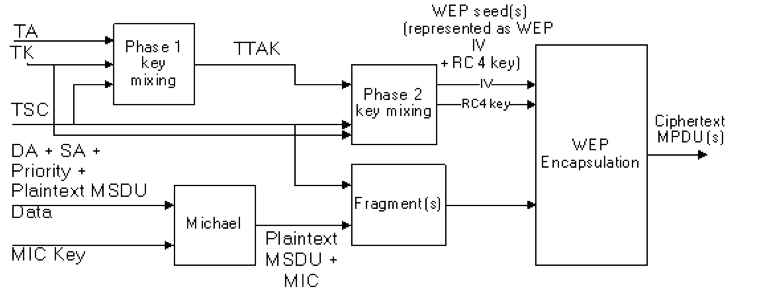
\includegraphics[width=\linewidth]{contents/background-in-wireless-networks/protected-network-standards/wpa/tkip/tkip-encapsulation-block-diagram.png}
    \caption{\gls{tkip} Encapsulation Block Diagram}
    {Source: \cite{ieee_80211_2020}}
    \label{figure:ieee80211_figure43c}
\end{figure}

Represented on Figure \ref{figure:ieee80211_figure43c}, the encryption process of \gls{tkip} combines the \gls{tk}, \gls{ta}, and \gls{tsc} using cryptographic mixing functions and uses it as the \gls{sk} and the \gls{iv} of the \gls{wep} algorithm, effectively enhancing the \gls{prng} seed strength by avoiding the reuse of keys. Then \gls{tkip} calculates the \gls{mic} by executing the Michael algorithm with the \gls{mic} key over the \gls{msdu} plaintext, priority, \gls{sa}, and \gls{da}. The result is fed to the original \gls{wep} algorithm, which outputs the \gls{mpdu} to be transmitted.

\begin{figure}[h]
    \centering
    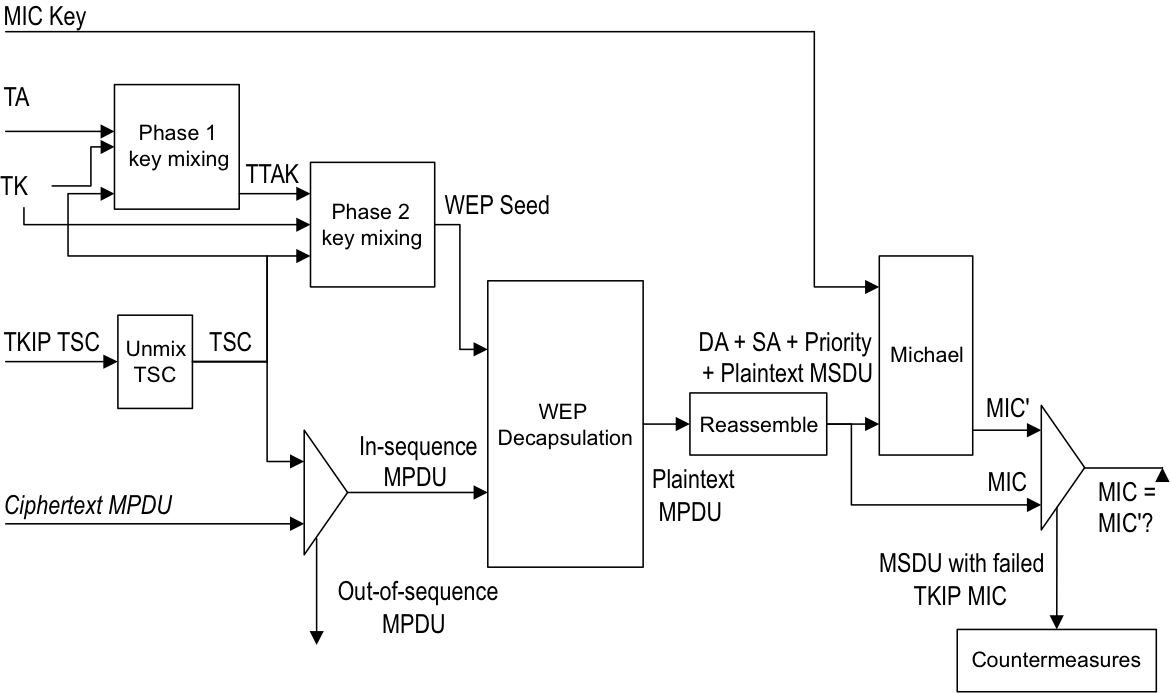
\includegraphics[width=\linewidth]{contents/background-in-wireless-networks/protected-network-standards/wpa/tkip/tkip-decapsulation-block-diagram.png}
    \caption{\gls{tkip} Decapsulation Block Diagram}
    {Source: \cite{ieee_80211_2020}}
    \label{figure:ieee80211_figure43d}
\end{figure}

When decrypting, \gls{tkip} rejects all \glspl{mpdu} received out of sequence. Then it calculates the \gls{wep} seed using the same mixing algorithm of the encryption process. The \gls{wep} algorithm is executed, decrypting the \gls{mpdu}. Michael is executed with the proper \gls{mic} key over the recently recovered data, the result is then compared to the \gls{mic} specified in the \gls{mpdu}. If the \glspl{mic} don't match, \gls{tkip} performs countermeasures procedures to mitigate what looks like an attack. Otherwise, the message is returned by the algorithm, meaning that the \gls{mpdu} was decrypted and successfully authenticated. The decryption mechanism is illustrated on Figure \ref{figure:ieee80211_figure43d}.

\FloatBarrier

\paragraph{Security}

A compromise was made on the \gls{tkip} design to make possible its use on legacy \gls{wep} hardware. The forgery attacks were mitigated with the introduction of the Michael algorithm, but, due to computing power constraints, while blocking the forged packets it would cause a denial of service on the network \cite{ieee_80211_2020}.

As \gls{tkip} just encapsulates the \gls{wep} algorithm, it still relies on the security of the \gls{rc4} \gls{prng}. It was found that the keystream generated by \gls{rc4} is biased towards certain sequences and it made practical attacks against \gls{wpa}-\gls{tkip} networks within an hour \cite{rc4nomore}. The attacker would establish a \gls{tcp} connection with some victim on the network and would repeatedly send identical packets particularly sized with a well-known content over the connection. Then the wireless traffic was captured and filtered to only what would likely be an attacker's packet. Ciphertext statistics were extracted and plaintext likelihoods calculated using a combination of the \gls{fm} and \gls{absab} biases. Finally, the \gls{mic} key is derived from one of the candidates with the correct \gls{icv}, allowing any other packet of the victim to be fully decrypted.


\subsubsection{WPA2}

In 2004, the \gls{ieee} 802.11i amendment was finalized and published and, as planned, the \gls{wifi} Alliance released a new protocol based on the document, \gls{wpa}2 \cite{wifi_state}. Unlike its predecessor, \gls{wpa}2 wasn’t designed to work with older hardware constraints and could provide more robust security mechanisms.

One of the key differences between \gls{wpa} and \gls{wpa}2 is its confidentiality and integrity protocol. On \gls{wpa} it was optional to have the new protocol implemented, while on \gls{wpa}2 its implementation is mandatory and \gls{tkip} should only be used as a fallback for interoperability with older devices.

\gls{wpa}2 relies on the same authenticators of \gls{wpa}, \gls{psk} for \gls{wpa}2-Personal and \gls{ieee} 802.1X for \gls{wpa}2-Enterprise.

\paragraph{CCMP}

The \gls{ccmp} uses the \gls{aes} block cipher operating in \gls{ccm} mode. \gls{ctr} provides data confidentiality, while \gls{cbc}-\gls{mac} is used for authentication and integrity. Originally, \gls{ccmp} supported only 128-bit \gls{aes} keys (\gls{ccmp}-128), but later revisions of the algorithm allowed the use of 256-bit keys (\gls{ccmp}-256) as well.

\begin{figure}[h]
    \centering
    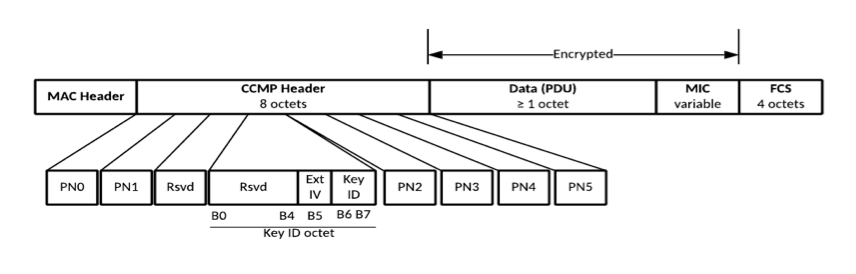
\includegraphics[width=\linewidth]{contents/background-in-wireless-networks/protected-network-standards/wpa2/ccmp/expanded-ccmp-mpdu.png}
    \caption{Expanded \gls{ccmp} \gls{mpdu}}
    {Source: \cite{ieee_80211_2020}}
    \label{figure:ieee80211_figure43n}
\end{figure}

Not needing to rely on \gls{wep} anymore, \gls{ccmp} unified the \gls{iv} field of \gls{wep} and \gls{eiv} field of \gls{wpa} into the 8-octet \gls{ccmp} Header field. The \gls{wep} \gls{icv} was dropped and the \gls{mic} field was turned into a variable size field, 8-octet or 16-octet long for \gls{ccmp}-128 and \gls{ccmp}-256 respectively. The resulting \gls{mpdu} is shown on Figure \ref{figure:ieee80211_figure43n}.

\begin{figure}[h]
    \centering
    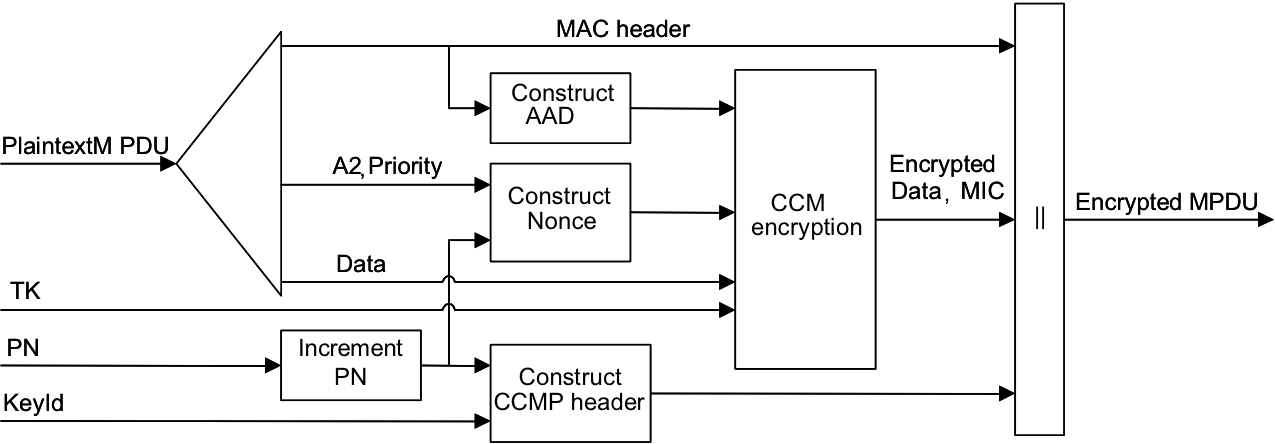
\includegraphics[width=\linewidth]{contents/background-in-wireless-networks/protected-network-standards/wpa2/ccmp/ccmp-encapsulation-block-diagram.png}
    \caption{\gls{ccmp} Encapsulation Block Diagram}
    {Source: \cite{ieee_80211_2020}}
    \label{figure:ieee80211_figure43o}
\end{figure}

On the encryption process, represented on Figure \ref{figure:ieee80211_figure43o}, \gls{ccmp} maintains a \gls{pn} value for each \gls{tk}, incrementing it sequentially for each \gls{mpdu} processed. The \gls{pn} is used along the \gls{kid} to build the \gls{ccmp} Header, part of the final \gls{mpdu}. \gls{pn} is also used together with the \gls{a2} and Priority of the \gls{mpdu} being consumed to calculate the Nonce Block, avoiding replay attacks. The \gls{mac} Header has its values authenticated by constructing the \gls{aad}, providing integrity protection. Finally, the \gls{ccm} Originator Processing is invoked with the values of \gls{aad}, nonce, plaintext, and \gls{tk} to form the ciphertext and the \gls{mic}. The encrypted \gls{mpdu} is accordingly assembled and sequentially transmitted.

\begin{figure}[h]
    \centering
    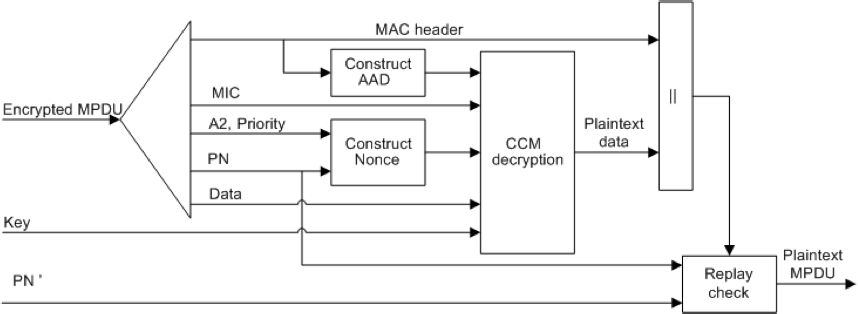
\includegraphics[width=\linewidth]{contents/background-in-wireless-networks/protected-network-standards/wpa2/ccmp/ccmp-decapsulation-block-diagram.png}
    \caption{\gls{ccmp} Decapsulation Block Diagram}
    {Source: \cite{ieee_80211_2020}}
    \label{figure:ieee80211_figure43r}
\end{figure}

To decrypt the \gls{mpdu}, the \gls{aad} is constructed in the same way as the original \gls{mpdu}. The Nonce Block uses the \gls{a2} and Priority values from \gls{mpdu} as usual, but it also gets the \gls{pn} from there. Then the \gls{ccm} Recipient Processing is invoked with the \gls{tk}, the calculated \gls{aad} and Nonce Block, and the extracted ciphertext and \gls{mic} values. The decrypted \gls{mpdu} is assembled with the resulting plaintext. Before having the \gls{mpdu} returned, the replay check is executed, which verifies if the extracted \gls{pn} value is less than or equal to the local \gls{pn} value for the \gls{tk}, implying a frame replay. The decryption process is shown on Figure \ref{figure:ieee80211_figure43r}.

\FloatBarrier

\paragraph{Security}

A compromise was made on the \gls{tkip} design to make possible its use on legacy \gls{wep} hardware. The forgery attacks were mitigated with the introduction of the Michael algorithm, but, due to computing power constraints, while blocking the forged packets it would cause a denial of service on the network \cite{ieee_80211_2020}.

As \gls{tkip} just encapsulates the \gls{wep} algorithm, it still relies on the security of the \gls{rc4} \gls{prng}. It was found that the keystream generated by \gls{rc4} is biased towards certain sequences and it made practical attacks against \gls{wpa}-\gls{tkip} networks within an hour \cite{rc4nomore}. The attacker would establish a \gls{tcp} connection with some victim on the network and would repeatedly send identical packets particularly sized with a well-known content over the connection. Then the wireless traffic was captured and filtered to only what would likely be an attacker's packet. Ciphertext statistics were extracted and plaintext likelihoods calculated using a combination of the \gls{fm} and \gls{absab} biases. Finally, the \gls{mic} key is derived from one of the candidates with the correct \gls{icv}, allowing any other packet of the victim to be fully decrypted.


\subsubsection{WPA3}

14 years after the \gls{wpa}2 release, \gls{wpa}3 was published. The new protocol is based on the \gls{ieee} 802.11-2016 revision and comes with a new handshake process that makes offline dictionary attacks impossible \cite{wpa3_spec}. \gls{wpa}3 retains interoperability with \gls{wpa}2 devices via the Transition Mode and must be supported by all \gls{wifi} devices certified since July 2020.

\paragraph{SAE}

The \gls{sae} protocol was originally defined on the \gls{ieee} 802.11s amendment for use on mesh networks \cite{ieee_80211_2020}. It is a variant of the Dragonfly Key Exchange \cite{rfc7664}, meant to provide an authentication mechanism resistant to offline brute-force attacks. \gls{sae} relies on discrete logarithm cryptography to achieve its security properties. The password derivation is made using one of the hash-to-curve functions specified in the protocol.

In the \gls{ieee} 802.11-2016 revision, the use of \gls{sae} was broadened to act as a replacement for the \gls{psk} authenticator of traditional wireless networks, allowing \gls{wifi} Alliance to define it as the authentication protocol for \gls{wpa}3-Personal networks \cite{wpa3_spec}.

\paragraph{GCMP}

The \gls{gcmp} is a more efficient alternative to \gls{ccmp} introduced in the \gls{ieee} 802.11ac amendment to allow devices to transfer data at higher speeds with less processing requirements \cite{ieee_80211_2020}. Just like \gls{ccmp}, it has a 128-bit (\gls{gcmp}-128) and a 256-bit (\gls{gcmp}-256) variants. \gls{wpa}3 enforces use of \gls{gcmp}-256 on \gls{wpa}3-Enterprise networks.

\begin{figure}[h]
    \centering
    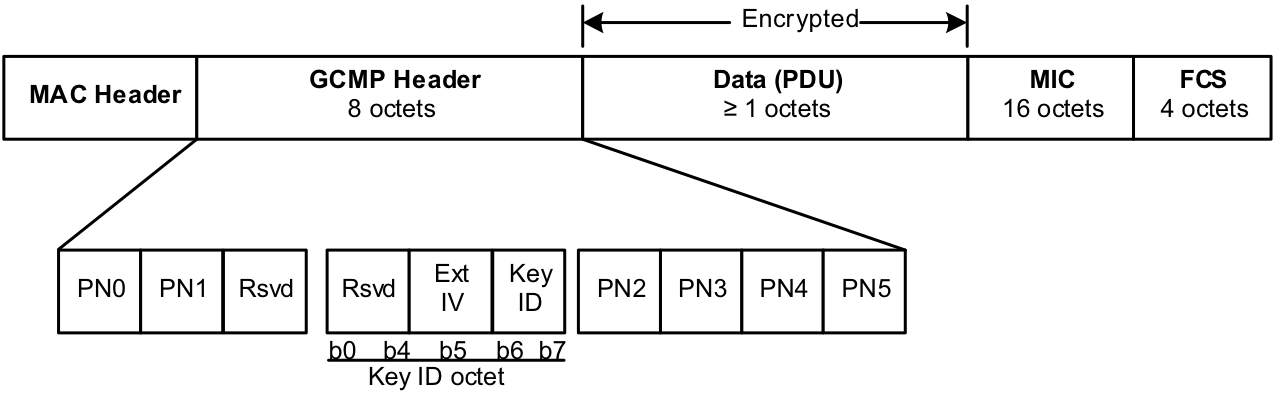
\includegraphics[width=\linewidth]{contents/background-in-wireless-networks/protected-network-standards/wpa3/gcmp/expanded-gcmp-mpdu.png}
    \caption{Expanded \gls{gcmp} \gls{mpdu}}
    {Source: \cite{ieee_80211_2020}}
    \label{figure:ieee80211_figure1226}
\end{figure}

Represented by Figure \ref{figure:ieee80211_figure1226}, the \gls{mpdu} of \gls{gcmp} is very similar to the \gls{ccmp} one, the \gls{mic} size being the only difference between them. Instead of a variant \gls{mic} size for 128-bit and 256-bit keys, \gls{gcmp}’s \gls{mic} is always 16-octet long.

\begin{figure}[h]
    \centering
    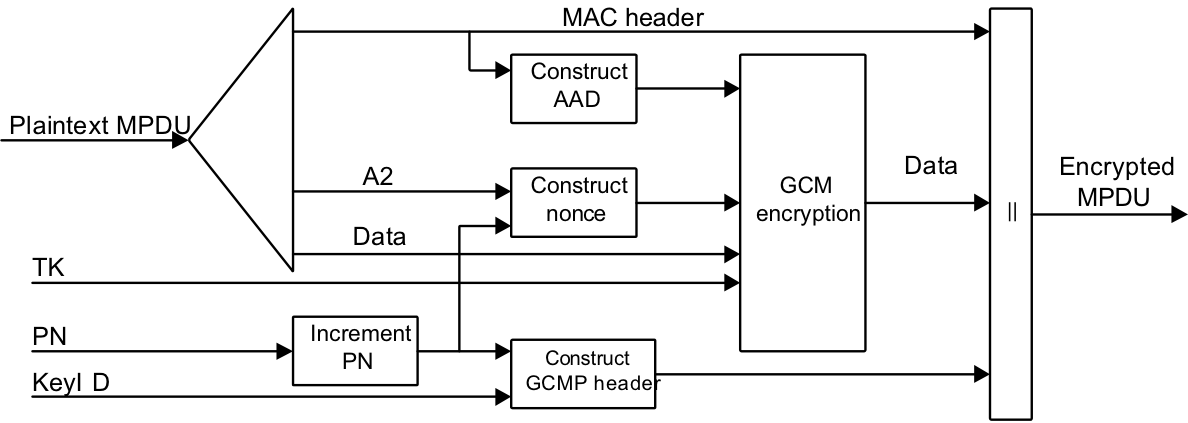
\includegraphics[width=\linewidth]{contents/background-in-wireless-networks/protected-network-standards/wpa3/gcmp/gcmp-encapsulation-block-diagram.png}
    \caption{\gls{gcmp} Encapsulation Block Diagram}
    {Source: \cite{ieee_80211_2020}}
    \label{figure:ieee80211_figure1227}
\end{figure}

The encapsulation process, shown on Figure \ref{figure:ieee80211_figure1227}, differs from \gls{ccmp} on the Nonce construction. The priority is no longer considered, only \gls{a2} and \gls{pn} still remain. As expected, the \gls{ccmp} Header construction is replaced with the \gls{gcmp} Header construction and the \gls{ccm} Originator Processing with the \gls{gcm} Originator Processing.

\begin{figure}[h]
    \centering
    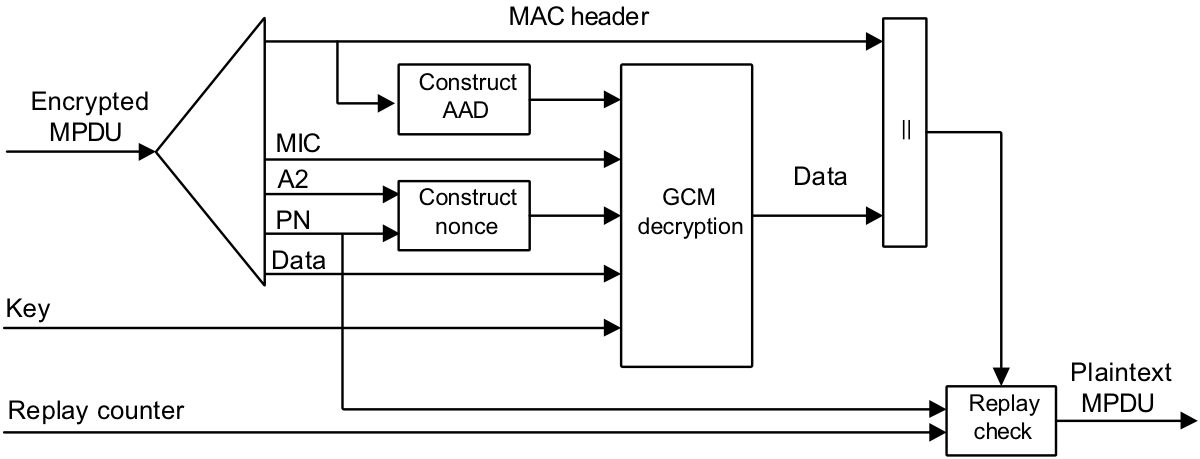
\includegraphics[width=\linewidth]{contents/background-in-wireless-networks/protected-network-standards/wpa3/gcmp/gcmp-decapsulation-block-diagram.png}
    \caption{\gls{gcmp} Decapsulation Block Diagram}
    {Source: \cite{ieee_80211_2020}}
    \label{figure:ieee80211_figure1229}
\end{figure}

On decapsulation, the \gls{ccm} Recipient Processing is substituted by the \gls{gcm} Recipient Processing. The Nonce construction is performed just like in the encapsulation process. The process is shown on Figure \ref{figure:ieee80211_figure1229}.

\FloatBarrier

\paragraph{Security}

A compromise was made on the \gls{tkip} design to make possible its use on legacy \gls{wep} hardware. The forgery attacks were mitigated with the introduction of the Michael algorithm, but, due to computing power constraints, while blocking the forged packets it would cause a denial of service on the network \cite{ieee_80211_2020}.

As \gls{tkip} just encapsulates the \gls{wep} algorithm, it still relies on the security of the \gls{rc4} \gls{prng}. It was found that the keystream generated by \gls{rc4} is biased towards certain sequences and it made practical attacks against \gls{wpa}-\gls{tkip} networks within an hour \cite{rc4nomore}. The attacker would establish a \gls{tcp} connection with some victim on the network and would repeatedly send identical packets particularly sized with a well-known content over the connection. Then the wireless traffic was captured and filtered to only what would likely be an attacker's packet. Ciphertext statistics were extracted and plaintext likelihoods calculated using a combination of the \gls{fm} and \gls{absab} biases. Finally, the \gls{mic} key is derived from one of the candidates with the correct \gls{icv}, allowing any other packet of the victim to be fully decrypted.



\subsection{Network Setup Standards}
\subsubsection{WPS}

Originally called \gls{wsc}, the \gls{wps} was introduced by Cisco in 2006 as an alternative authentication method for \gls{wpa} networks. The main goal of this protocol is "to simplify the security setup and management of wireless networks" at home, allowing a client to acquire network credentials with the \gls{pbc}, by typing a \gls{pin}, or via \gls{nfc} \cite{wps_spec}.

When \gls{wps} is configured to authenticate with a \gls{pin}, it uses an 8-digit number. The last digit of the \gls{pin} is a checksum of the first 7 digits, so there are \( 10^7 \) possible \gls{pin}s, too many to be brute-forced online. But in 2011 a researcher discovered that \gls{wps} reported the correctness of the first and last 4-digits of the \gls{pin} individually, making it possible to gain access to the network in, at most, \( 10^4 + 10^3 \) attempts \cite{viehboeck}. This flaw was fixed on version 2.0.2 of \gls{wps} \cite{wps_spec}.

In 2014, a problem in the implementation of \gls{wps} by several vendors made it feasible to perform an offline brute-force attack \cite{pixiedust}. The lack of entropy allowed the state of the internal \gls{prng} to be derived from information retrieved by partially executing the \gls{wps} protocol on the victim, making it possible to compute the E-S1 and E-S2 nonces and subsequently brute-force the \gls{pin}. The E-S1 and E-S2 nonces are 128 random bits sent by the \gls{ap} to the \gls{sta} that are used to salt the first and second parts of the \gls{pin} before hashing it.

\subsubsection{WEC}

Intended to replace \gls{wps}, the \gls{wec} protocol uses, mainly,  \gls{qr} codes or \gls{nfc} tags to establish the network connection between the client and the station \cite{wec_spec}. It was designed with \gls{iot} devices in mind, standardizing the onboarding process and making it possible to change wireless configurations without having to re-join all devices to the network.

The protocol relies on asymmetric cryptography to create a secure channel between the peers to exchange the credentials. Unlike \gls{wps}, there is no \gls{pin} and an attacker is not able to take advantage of a legitimate authentication initiation to acquire network credentials.


